\documentclass[11pt,xcolor=table]{beamer}

\usetheme[progressbar=frametitle]{metropolis}
\usepackage{appendixnumberbeamer}
\usepackage{pgfpages}
%\setbeameroption{show notes on second screen}
  \setbeamertemplate{enumerate items}[square]
\usepackage{multirow}

\usepackage{graphicx}

\usepackage{xcolor}

\newcommand{\link}[3][mLightBrown]{\href{#2}{\color{#1}{#3}}}%


\newcommand{\questionslide}[0]{
{\setbeamercolor{palette primary}{fg=black, bg=yellow}
\begin{frame}[standout]
    \raggedright
  Any questions? \\ \vspace{1cm}
  \raggedleft
  \dots{ } Remember -- Every question is useful!
\end{frame}
}}

\newcommand{\task}[1]{
   \begin{alertblock}
   {\centering \vspace{-1.5ex} \\ #1  \\ \vspace{-1.5ex} }
   \end{alertblock}
   }

\setbeamercolor{block title alerted}{%
    use={block title, alerted text},
    bg=yellow,
    fg=black
}

\definecolor{peppermint}{RGB}{75, 161, 115}
%\definecolor{peppermint}{RGB}{75, 161, 115}


\setbeamercolor{alerted text}{fg=peppermint , bg= black}

\usepackage{booktabs}
\usepackage[scale=2]{ccicons}

\usepackage{pgfplots}
\usepgfplotslibrary{dateplot}

\makeatletter 
\def\beamer@framenotesbegin{% at beginning of slide
    \usebeamercolor[fg]{normal text}
    \gdef\beamer@noteitems{}% 
    \gdef\beamer@notes{}% 
}
\makeatother


\usepackage{xspace}
\newcommand{\themename}{\textbf{\textsc{metropolis}}\xspace}

\title{Exercises and Questions around IV
}
\subtitle{Econ 140, Section 10}
% \date{\today}
\date{}
\author{Jonathan Old}

% \titlegraphic{\hfill\includegraphics[height=1.5cm]{logo.pdf}}

\begin{document}

\maketitle

\begin{frame}{Roadmap}
  \setbeamertemplate{section in toc}[sections numbered]
  \tableofcontents%[hideallsubsections]
\end{frame}







\section{Recap: IV}


\begin{frame}{Recap: IV summary}

We need the following three assumptions for IV to work: 
    \begin{enumerate}
    \item \textbf{Relevance}: $Z$ must truly affect $X$
    \item \textbf{Independence/Exogeneity}: $Z$ is as good as randomly assigned
    \item \textbf{Exclusion Restriction}: The \textbf{only} way that $Z$ affects $Y$ is via $X$.
    \end{enumerate}



    \begin{figure}
 
        \centering
        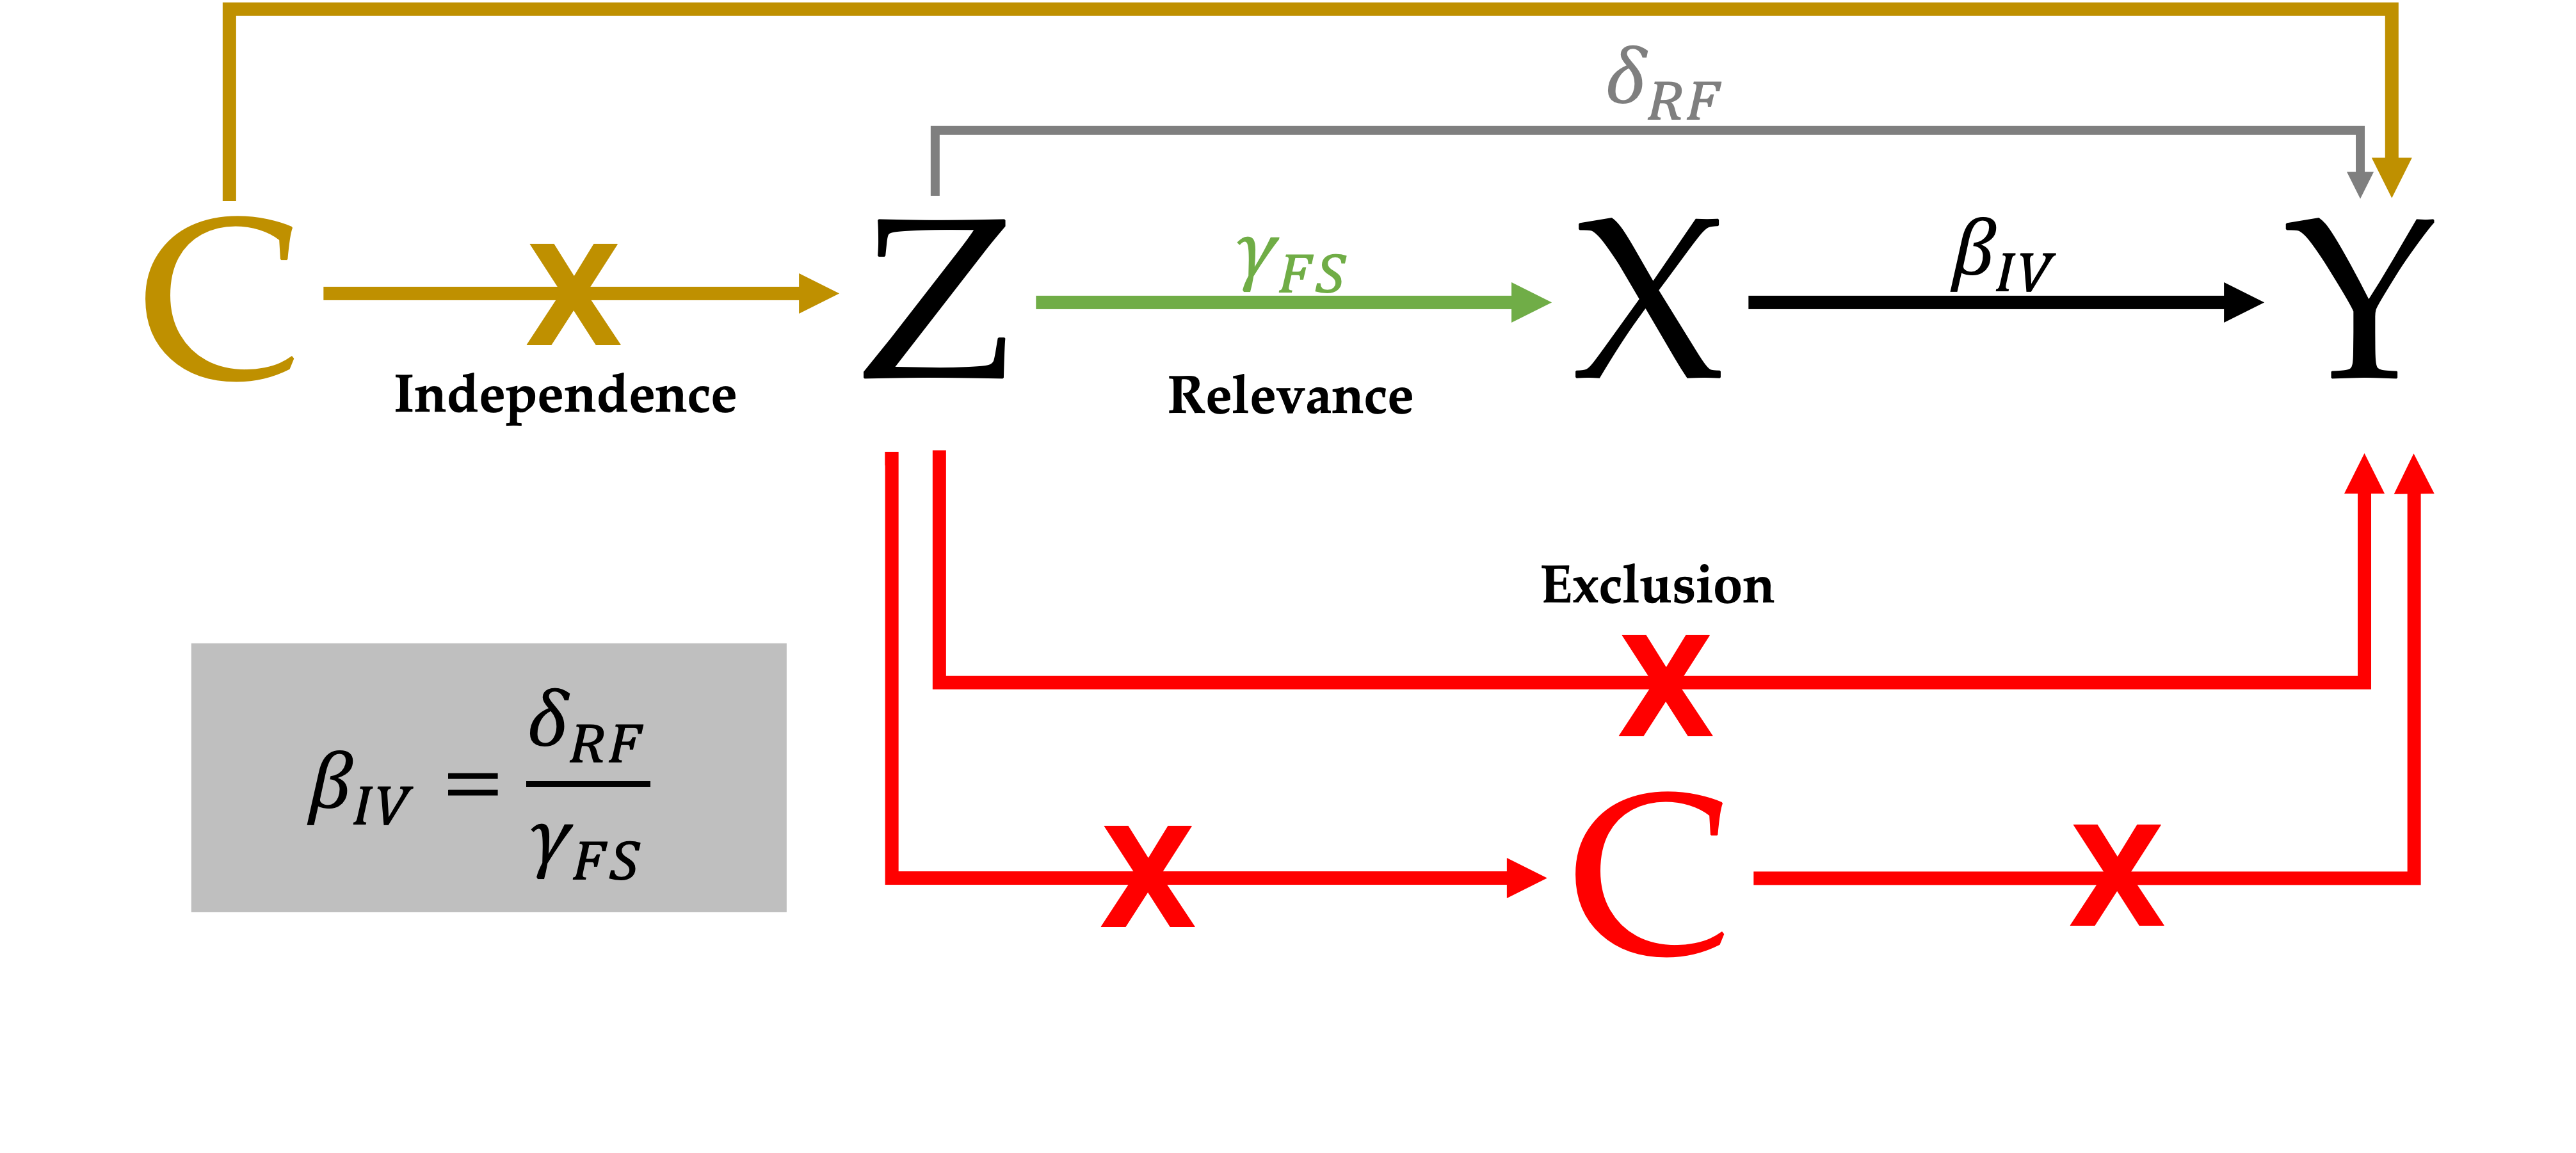
\includegraphics[width=1\textwidth]{DAGs/iv_summary_full.png}
        %\caption{Almost all you need to know about IVs!}
        \label{fig:iv3}
    \end{figure}
    
   \end{frame}






\begin{frame}{How IV estimates can be different from OLS estimates}
    \begin{itemize}
        \item \textbf{OVB:} If OLS had omitted variable bias, and our instrument is valid, then the IV estimate should be different. We can check whether this is plausible with the OVB formula
        \item \textbf{Measurement error:} If we have random measurement error in the independent variable ($X$), then we can use IV to overcome this. In that case, the IV coefficient will be larger (in absolute value) than the OLS coefficient
        \item \textbf{LATE:} OLS gives us  ATT + Selection Bias, while IV gives us the treatment effect on the compliers (LATE). The ATT may be different from LATE, even without selection bias.
        \item \textbf{Invalid IV:} Hard to determine  what exactly is going on
        \item \textbf{Sampling variation}: This can just happen by chance
        
    \end{itemize}
    
\end{frame}











\begin{frame}{IV and controls}
    \begin{itemize}
        \item There is a catch in IV: independence (exogeneity) and exclusion restriction only need to hold \textbf{conditionally}
        \item This means: If we \textbf{know} C, we can control for it in the IV regression, and the concerns go away
        \item But then, we have the old OLS problems again
        \item So we should only do this in cases where we really know all the C's.    
    \end{itemize}
    
\end{frame}






\section{Group work}

\begin{frame}{Group work}

    \begin{itemize}
    
    
\item[\textit{Group 1:}] We are interested in the effect of being in the army on crime. We instrument being in the army with a lottery (\link{https://www.aeaweb.org/articles?id=10.1257/app.3.2.119}{paper})
%\item[\textit{Group 2:}]  We are interested in the effect of protestant religion on economic growth. We instrument protestantism in a region with the distance to Wittenberg (\link{https://academic.oup.com/qje/article/124/2/531/1905076}{paper})

\item[\textit{Group 2:}]  We are interested in the effect of income on conflict. We instrument income with rainfall (\link{https://www-journals-uchicago-edu.libproxy.berkeley.edu/doi/10.1086/421174}{paper})


\item[\textit{Group 3:}]  We are interested in the effect of air pollution on mortality. We instrument local air pollution with wind direction (\link{https://www.aeaweb.org/articles?id=10.1257/aer.20180279}{paper})


       \end{itemize}

\begin{enumerate}
	\item Relevance: Z must truly affect X
	\item Independence/Exogeneity: Z is as good as randomly assigned
	\item Exclusion restriction: The \textbf{only} way that Z affects Y is via X
\end{enumerate}

%\textbf{\alert{Your job: Discuss whether these three assumptions hold!!}}

 %  \begin{alertblock} {\centering \vspace{-1.5ex} \\ Your job: Discuss whether these three assumptions hold!  \\ \vspace{-1.5ex} } \end{alertblock}
    
    \task{Your job: Discuss whether these assumptions hold!}
   \end{frame}










\section{IV Exam Exercise}

\begin{frame}[allowframebreaks]{IV Exam exercise}
The land of Econometrea consists of 34 islands. Each island has their own university and students attend uni on their home island. Students in Econometrea either have to attend lectures in person or watch them online. Priyanka has obtained data for the students from all the universities and would like to study the effect of watching lectures online on the students’ exam scores. For each student she has the exam score (0 - 100, 70+ is a first, 40 and below a fail), which she uses as her left hand side variable, the fraction of lectures watched online, and how on how many days the student visited the library each week. Priyanka obtains the following regression results:\\

\framebreak 
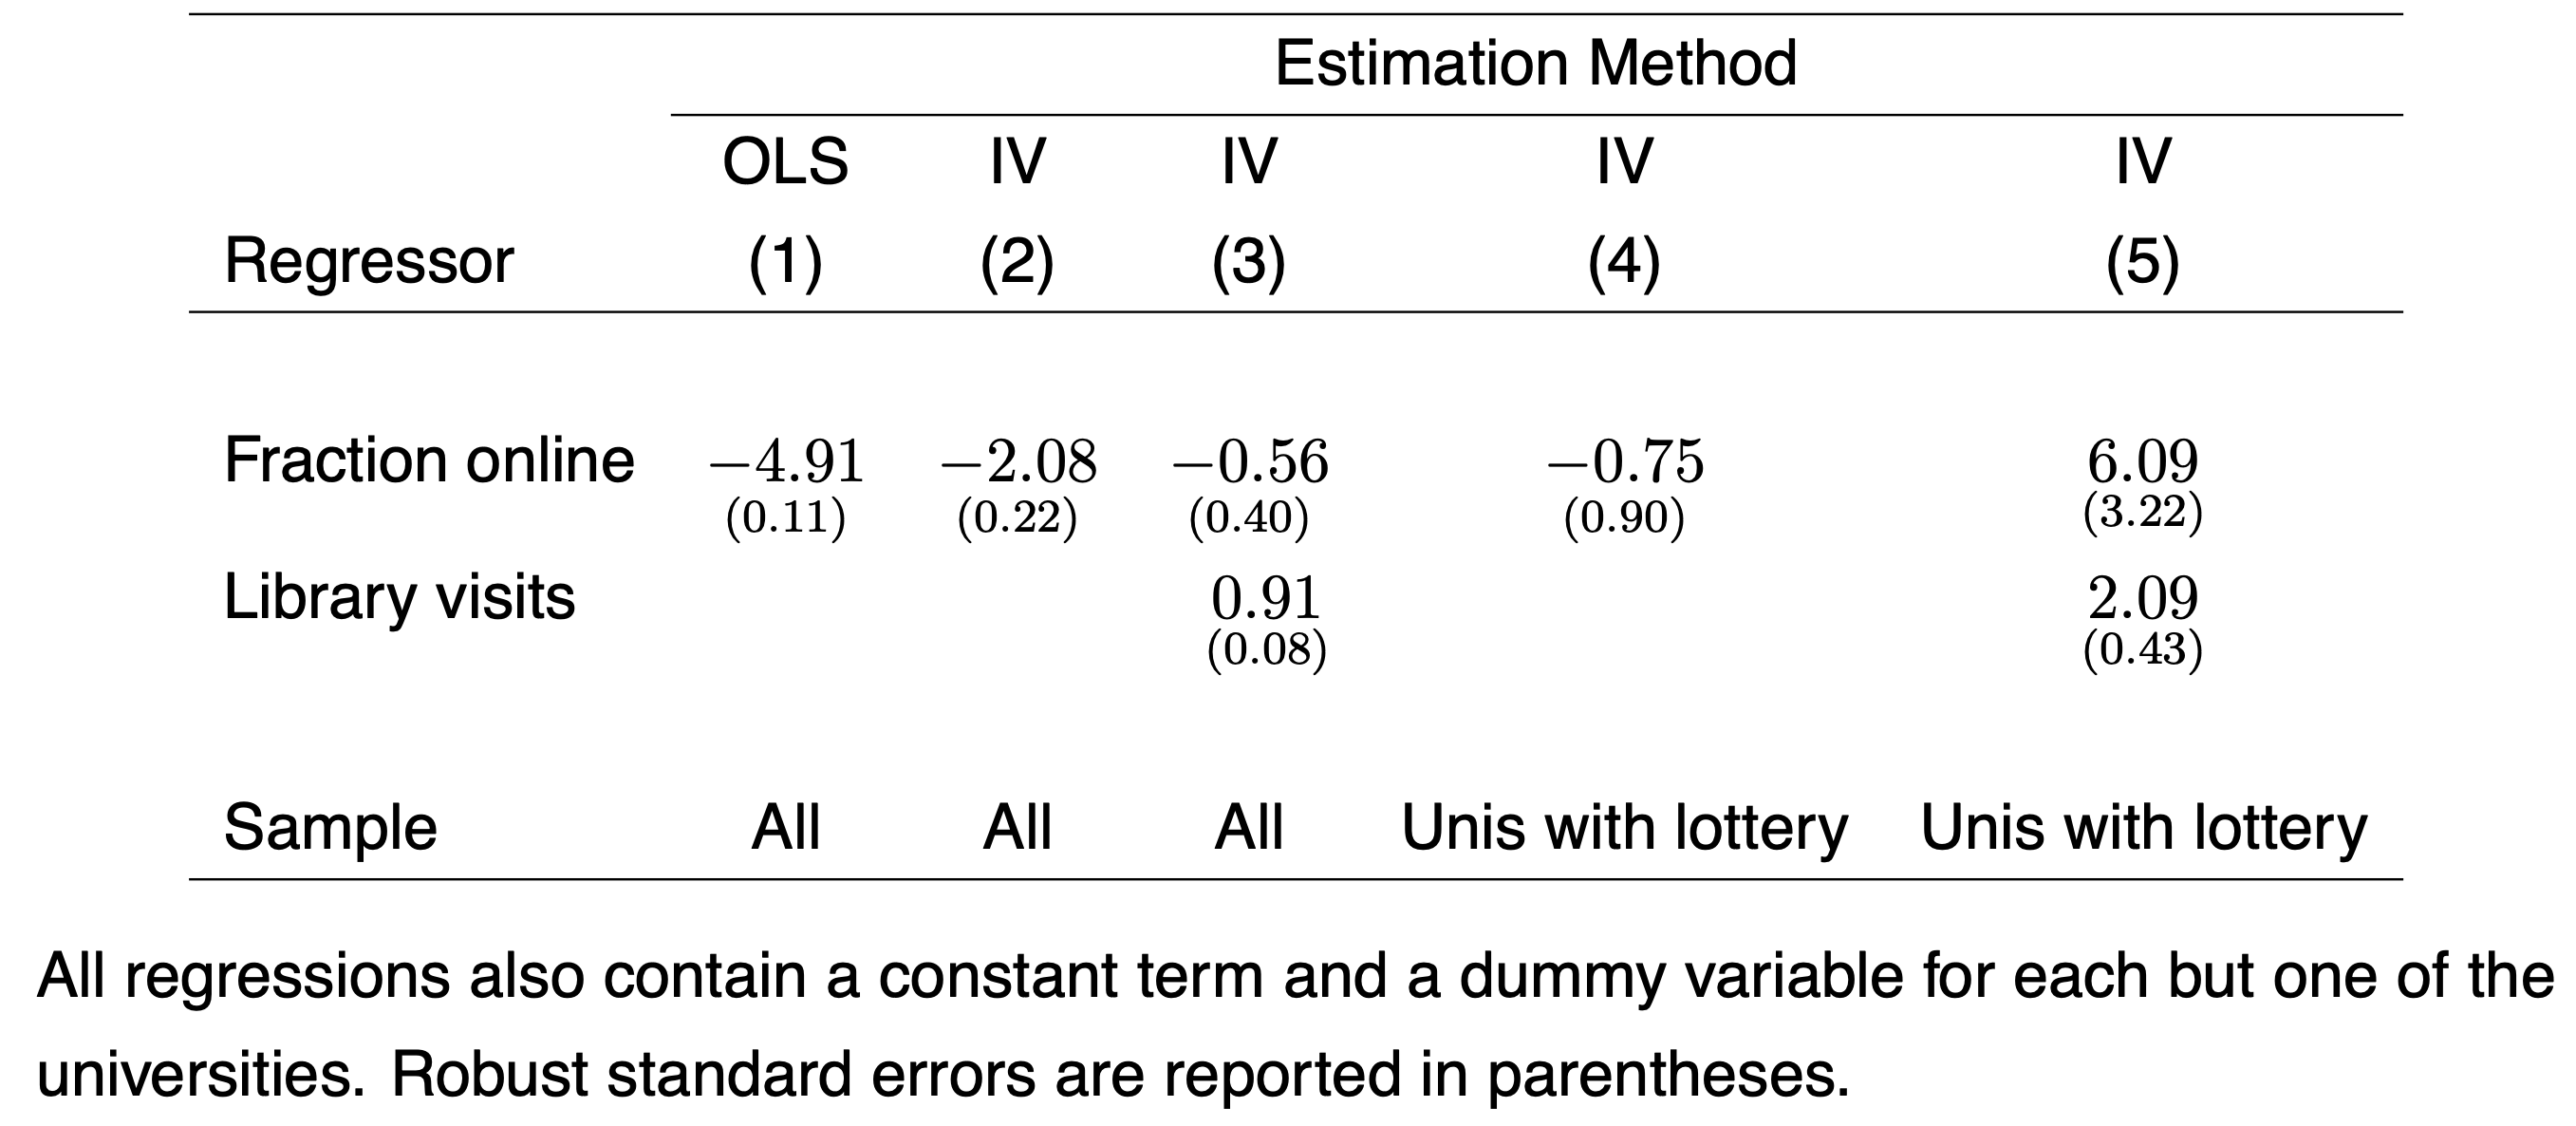
\includegraphics[width=1.0\textwidth]{tables/IV_Table.png}

\framebreak
(a) What is the interpretation of the coefficient in column (1). If this were a causal effect, would it be big or small? Explain whether this estimate is likely to have a causal interpretation.\\

(b) Wei Min observes that some halls of residence are close to the lecture rooms while others are further away and suggests to use the distance of halls from lecture halls as an instrumental variable for the fraction of lectures watched online. Results are in column (2). Explain which assumptions need to be satisfied for the IV to deliver better causal estimates than OLS here. Discuss the validity of the assumptions in this case.
\framebreak 
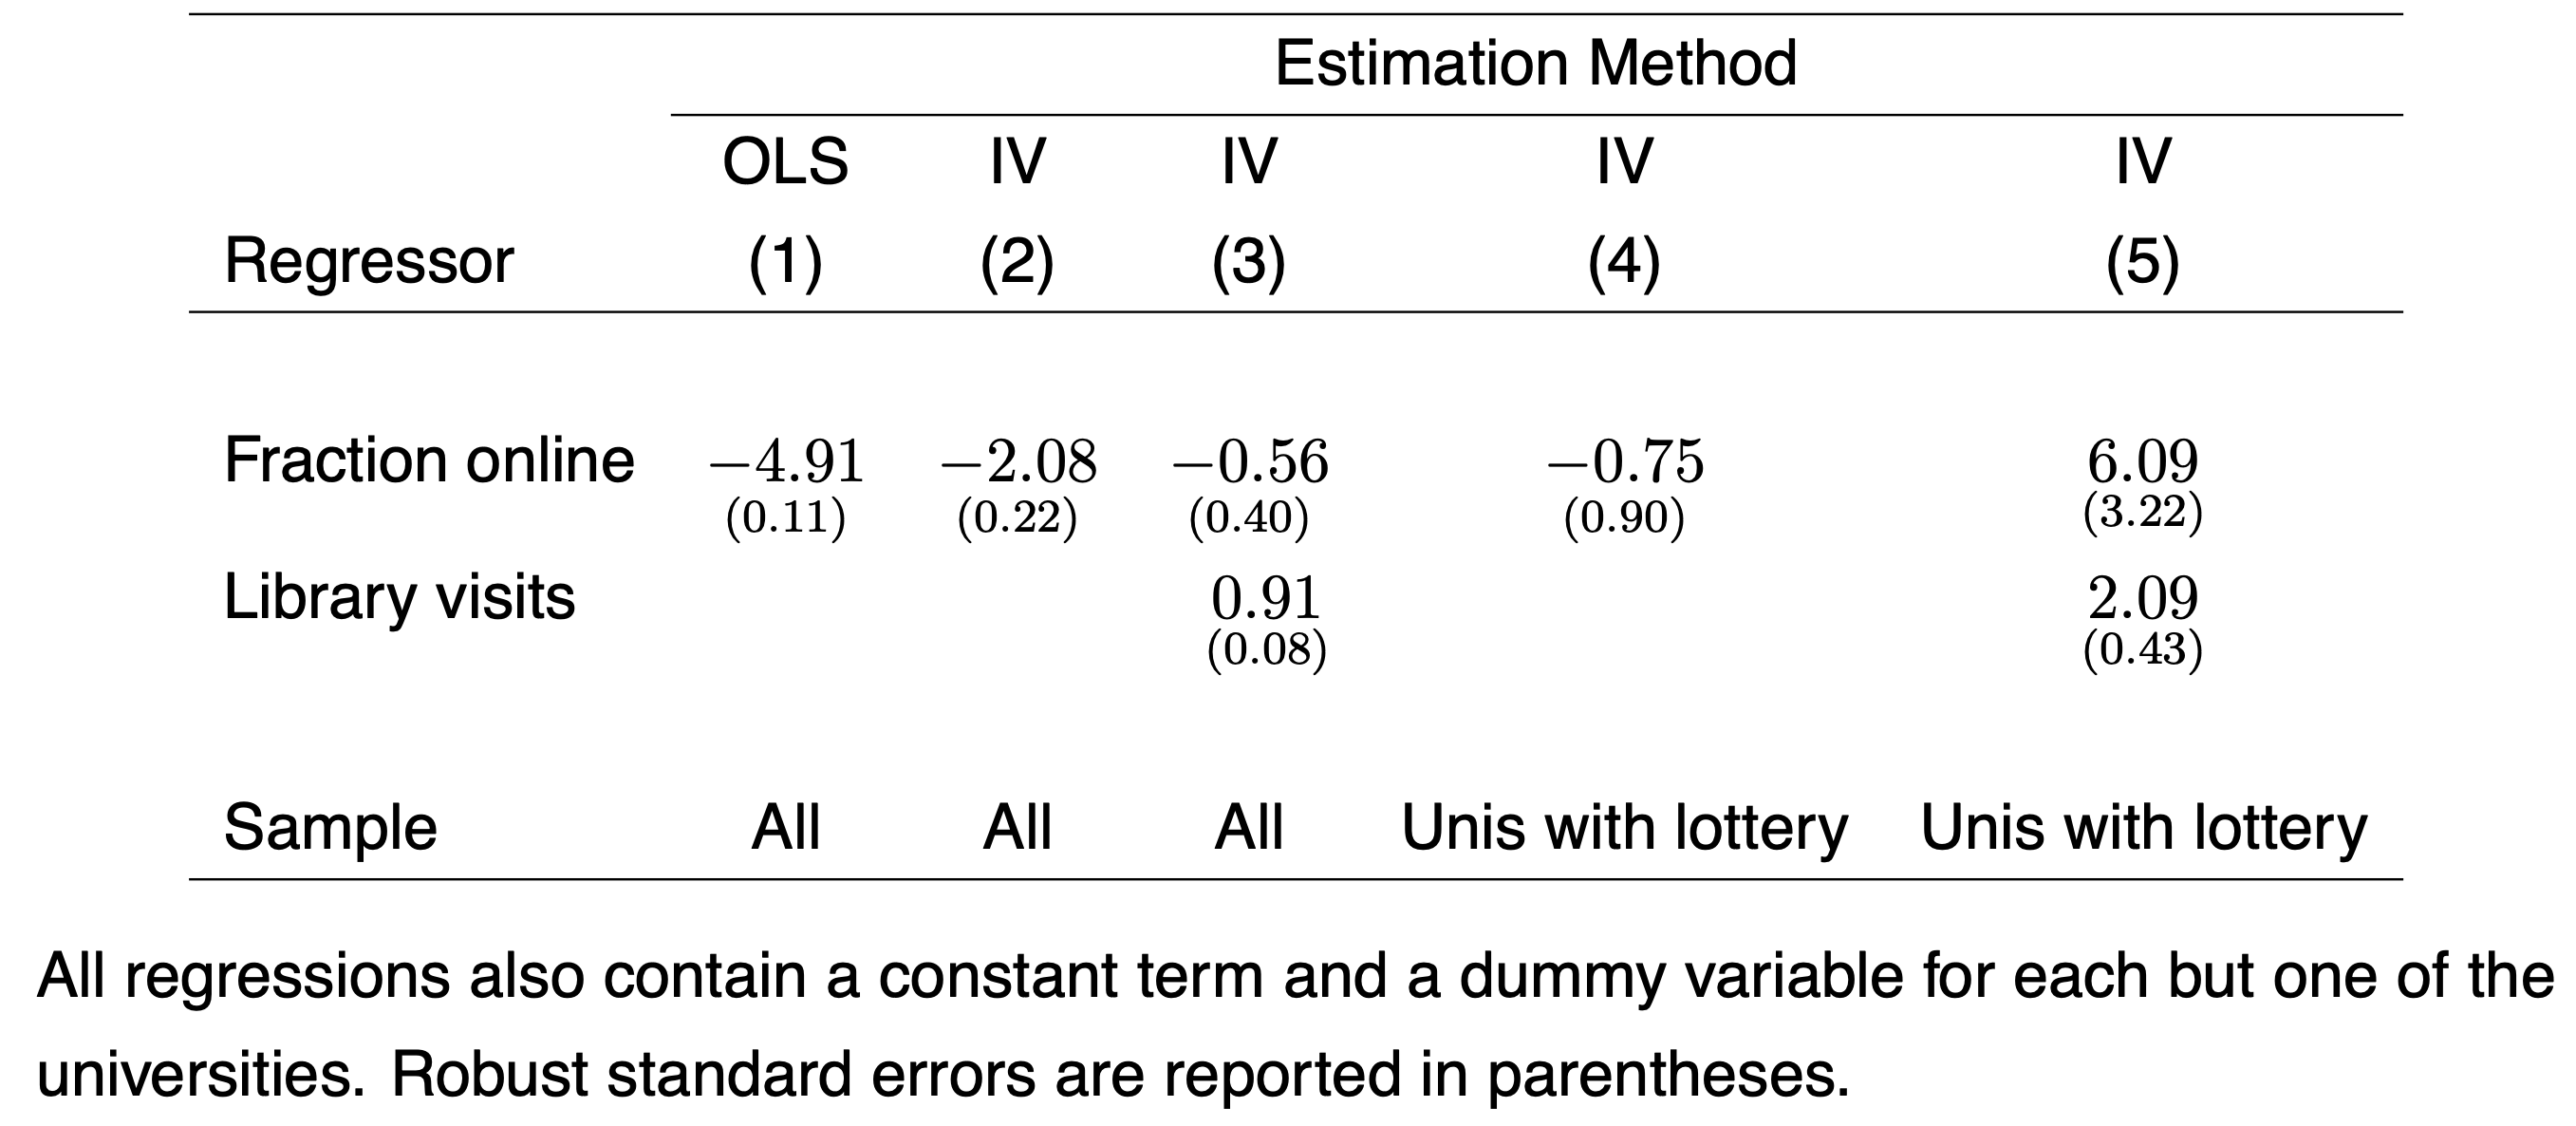
\includegraphics[width=0.9\textwidth]{tables/IV_Table.png}
\framebreak

\alert{Solution}
\begin{itemize}
    \item Students who watch all lectures online, on average, have around 4.9 fewer points on the exam than students who went to all lecturs in person. This is a moderately strong effect, but likely not causal (think of omitted variables, such as student motivation)
\end{itemize}
\framebreak

\alert{Solution}
    \begin{itemize}
    \item \textbf{Relevance:} Proximity to lecture halls must correlate strongly with lecture attendance. This is plausible from our experience, and we could test this using an F-test.
    \item  
    \textbf{Independence/Exogeneity:}  Proximity must be as good as randomly allocated. This might not hold here, for example, if more motivated students live closer to campus.
    \item
    \textbf{Exclusion restruction:} Proximity to lecture halls only influences exam scores because it has an effect on lecture attendance. This can be violated if proximity also affects the probability to go and study in the library, or if residence halls closer to campus are also closer to bars
\end{itemize}

\framebreak
(c) Alma points out to Wei Min that students can pick which hall they want to live in and that some halls are located in Study Village, close to lecture halls and the library while others are located further away in Party Town, surrounded by pubs. How does this information affect your assessment of the IV strategy?\\
(d) Manuel realises that the data also include a variable for the number of times a student has checked into the library per week. He suggests to rerun the instrumental variables regression adding this variable as a control. Results for this regression are displayed in column (3). Assess Manuel’s strategy.

\framebreak 
\alert{Solution}
\begin{itemize}
    \item This would be a violation of independence/exogeneity: The students who live closer to the campus are just inherently different than students who live far away
    \item Library visits are a bad control: They are another outcome of the instrument, and so controlling for them introduces additional bias.
\end{itemize}

\framebreak 
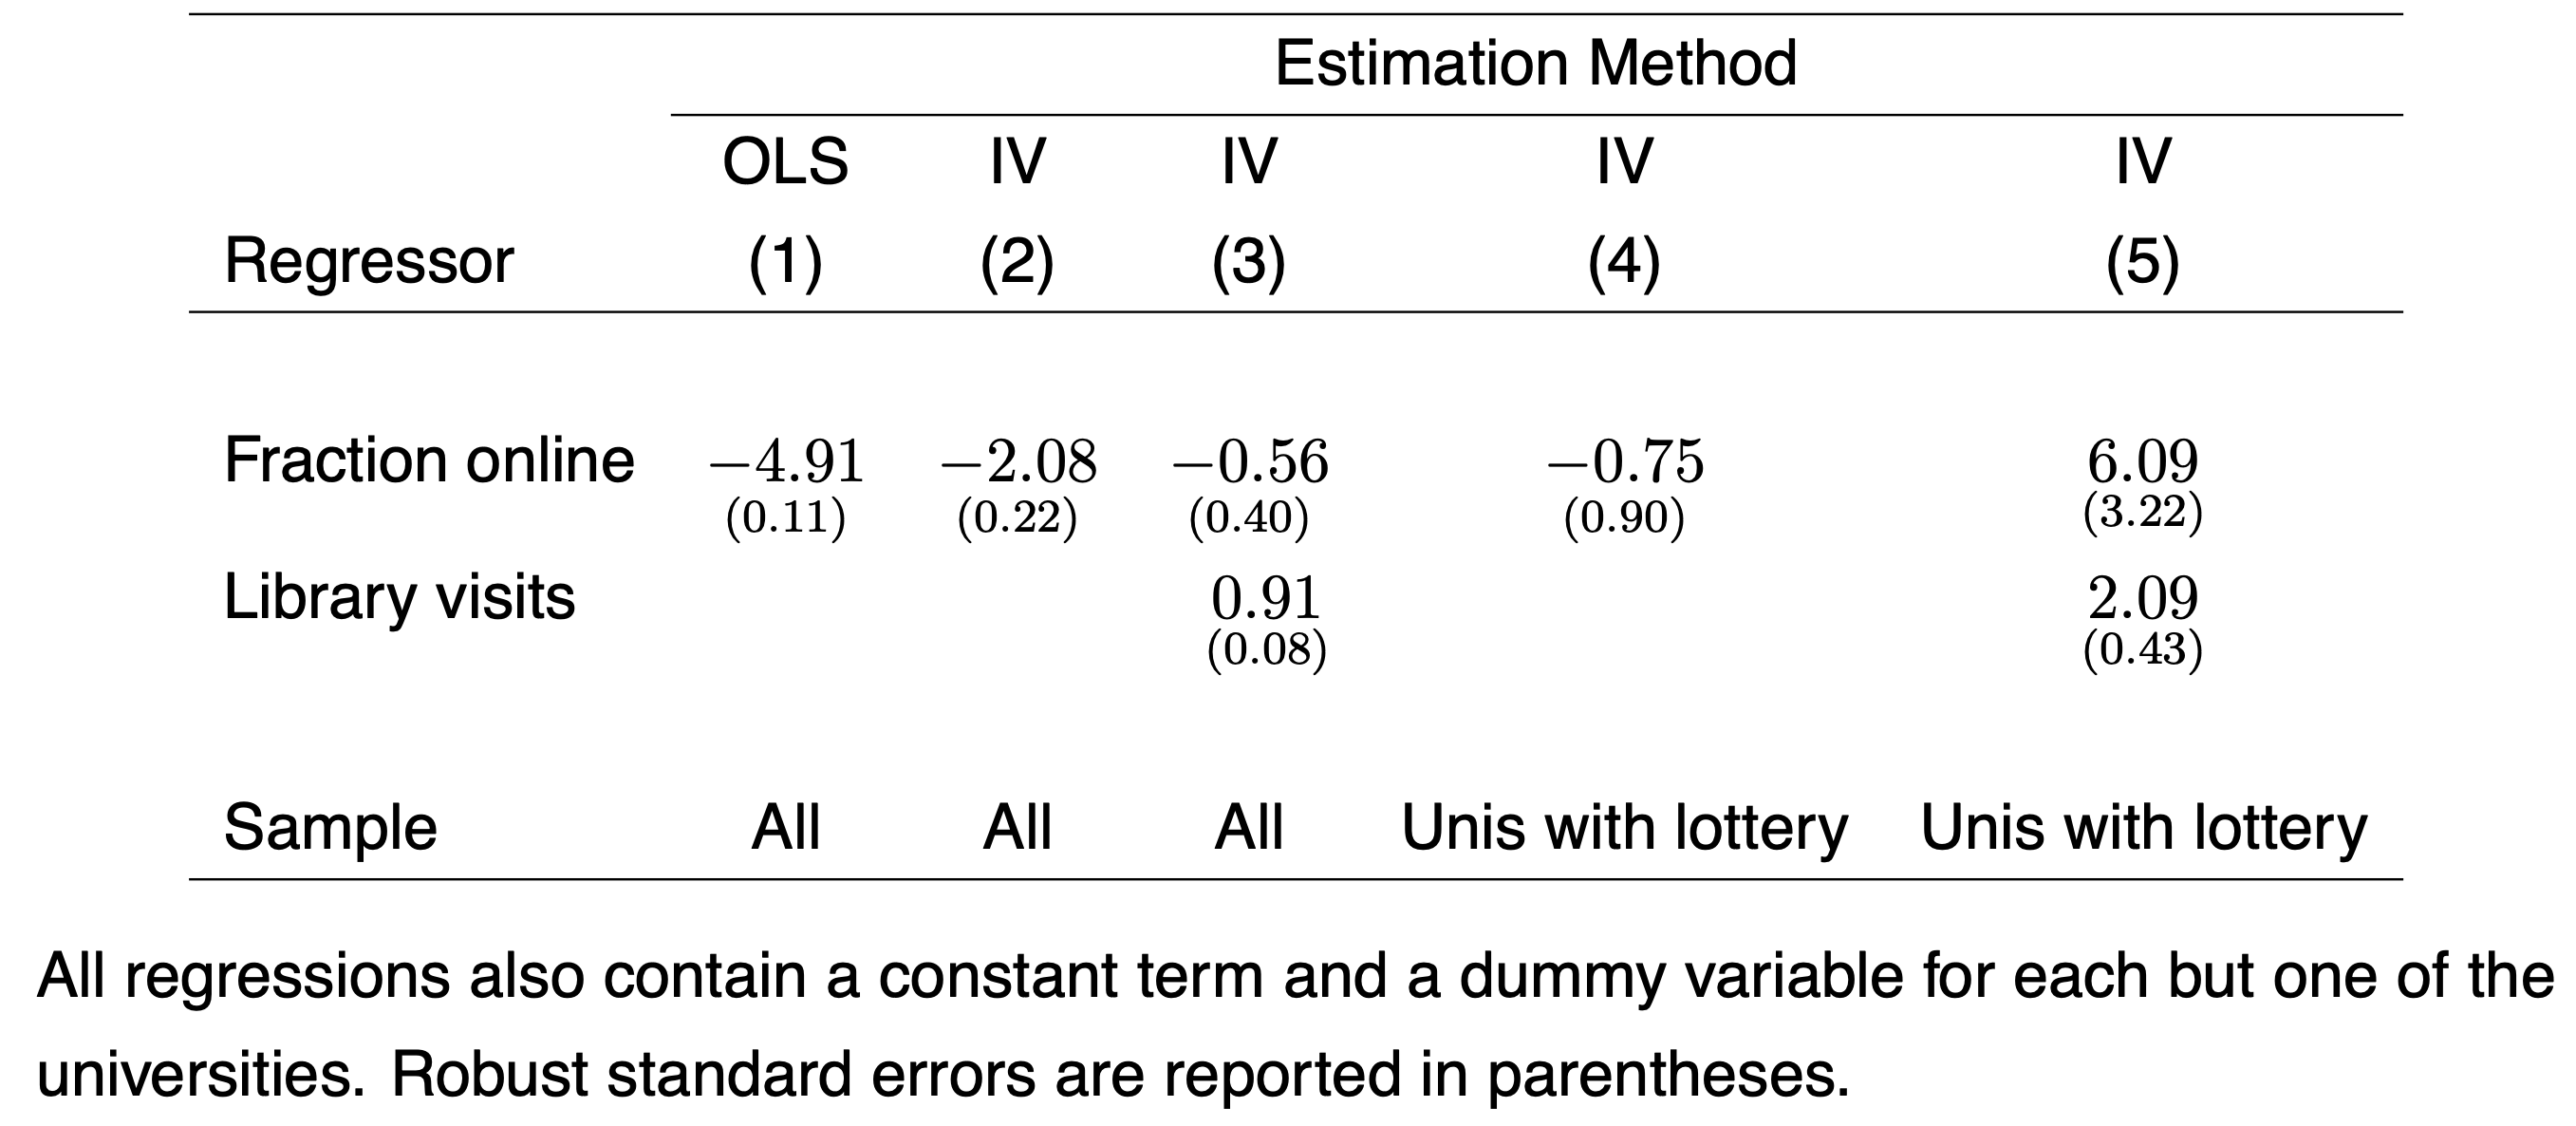
\includegraphics[width=1.0\textwidth]{tables/IV_Table.png}

\framebreak 


(e) Jenny notices that there are five universities which assign students to their halls of residence by a lottery. She suggests to run the IV model from columns (2) and (3) for the subsample of students from these universities only. Results are displayed in columns (4) and (5). Assess Jenny’s regressions.\\

(f) Drawing on the results in the table above, what have you learned from this exercise about the causal effect of watching lectures online on students’ exam results?


\framebreak 
\alert{Solution}
\begin{itemize}
    \item For these universities, the distance is as good as randomly assigned, and so we have no violations of the independence/exogeneity restriction. However, the exclusion restriction may still not hold.
    \item In a simply OLS regression, it may look as if watching lectures online causes worse grades. However, we can correct for this using a valid IV, and find that the effect is only very small and statistically insignificant.
\end{itemize}


\end{frame}




\section{Questions}



























\end{document}
